\documentclass{article}
\usepackage{amsmath,amssymb,amsthm,graphicx,tikz}

\newcommand{\E}{\mathbb{E}}
\newcommand{\Var}{\operatorname{Var}}
\DeclareMathOperator{\plim}{plim}

\newtheorem{theorem}{Theorem}
\newtheorem{assumption}{Assumption}

\title{The Effect of Minimum Wage Increases on Local Unemployment: A Synthetic Control Approach\thanks{The authors thank the Department of Economics at the University of Georgia for thoughtful comments. All errors are our own.}}
\author{Hugo Sant'Anna\thanks{Collat School of Business, University of Alabama at Birmingham. Email: hsantanna@uab.edu.} \quad Samyam Shrestha\thanks{Department of Economics, University of Georgia. Email: samyam@uga.edu.}}
\date{\today}

\begin{document}
\maketitle

\begin{abstract}
This paper estimates the causal effect of minimum wage increases on local unemployment using the synthetic control method. Exploiting variation in the timing and magnitude of state-level minimum wage hikes between 2010 and 2023, we construct synthetic counterfactuals for treated states. We find that a \$1 increase in the minimum wage leads to a 0.3--0.5 percentage point increase in the unemployment rate among workers aged 16--24, with effects concentrated in the retail and food services sectors. The aggregate unemployment effect is small and statistically insignificant, consistent with the monopsony model of low-wage labor markets.
\end{abstract}

\section{Introduction}

The minimum wage remains one of the most debated instruments in labor economics. Since \citet{card1994minimum}, the empirical consensus has shifted from the textbook prediction of unambiguous disemployment effects toward a more nuanced view in which labor market structure---particularly monopsony power---mediates the employment response.

We contribute to this literature by applying the augmented synthetic control method of \citet{ben2021augmented} to a panel of U.S.\ states observed quarterly from 2008 to 2023. Our identification strategy exploits 47 state-level minimum wage changes during this period.

\subsection{Related Literature}

The modern minimum wage literature begins with \citet{card1994minimum}, who found no significant employment effects from New Jersey's 1992 minimum wage increase. Subsequent work by \citet{dube2010minimum} generalized this finding using contiguous county pairs. On the other side, \citet{neumark2014revisiting} argue that longer-run adjustments reveal meaningful disemployment.

\section{Model}

Consider a labor market with $N$ firms, each with some degree of monopsony power. Firm $j$ faces an upward-sloping labor supply curve:
$$L_j^s(w) = \alpha_j + \beta_j w + \varepsilon_j,$$
where $w$ is the wage and $\varepsilon_j$ captures idiosyncratic supply shocks. The firm's profit maximization problem is:
\begin{equation}
  \max_{L_j} \; f(L_j) - w(L_j) \cdot L_j,
  \label{eq:profit}
\end{equation}
where $f(\cdot)$ is the production function and $w(L_j)$ is the inverse labor supply. The first-order condition yields the standard monopsony markup:
\begin{align}
  f'(L_j^*) &= w(L_j^*) \left(1 + \frac{1}{\eta_j}\right) \\
  &= w(L_j^*) + \frac{w(L_j^*)}{\eta_j},
\end{align}
where $\eta_j$ is the firm-level labor supply elasticity.

\begin{assumption}
The labor supply elasticity $\eta_j > 0$ is finite for all firms, implying imperfect competition.
\end{assumption}

\begin{theorem}
Under Assumption~1, a binding minimum wage $\bar{w} \in (w^*, w^m)$ increases employment, where $w^*$ is the competitive wage and $w^m$ is the monopsony wage.
\end{theorem}

\section{Data}

We use the Current Population Survey (CPS) merged with state minimum wage legislation data from the Department of Labor. Table~\ref{tab:summary} reports summary statistics for the treatment and control groups.

\begin{table}[htbp]
\centering
\caption{Summary Statistics by Treatment Status}
\label{tab:summary}
\begin{tabular}{lccc}
\hline
Variable & Treated & Control & Difference \\
\hline
Unemployment rate (\%) & 5.8 & 5.2 & 0.6 \\
Youth unemployment (\%) & 14.3 & 12.1 & 2.2 \\
Minimum wage (\$) & 10.50 & 7.25 & 3.25 \\
Median household income (\$) & 62,400 & 55,800 & 6,600 \\
Population (millions) & 8.4 & 5.1 & 3.3 \\
\hline
\end{tabular}
\end{table}

\section{Empirical Strategy}

The synthetic control estimator constructs weights $\mathbf{w} = (w_1, \ldots, w_J)'$ to minimize the pre-treatment prediction error:
\[
  \min_{\mathbf{w}} \sum_{t=1}^{T_0} \left( Y_{1t} - \sum_{j=2}^{J+1} w_j Y_{jt} \right)^2 \quad \text{s.t.} \quad w_j \geq 0, \; \sum_j w_j = 1.
\]
The treatment effect at time $t > T_0$ is then:
\begin{equation}
  \hat{\tau}_t = Y_{1t} - \sum_{j=2}^{J+1} \hat{w}_j Y_{jt}.
  \label{eq:tau}
\end{equation}

We assess statistical significance using permutation inference: we iteratively reassign treatment to each donor unit and compare the treated gap to the distribution of placebo gaps.

\section{Results}

Our main results are as follows:

\begin{itemize}
  \item The aggregate unemployment effect of a \$1 minimum wage increase is 0.1 percentage points (s.e.\ 0.08), statistically insignificant.
  \item Youth unemployment (ages 16--24) increases by 0.4 percentage points (s.e.\ 0.15), significant at the 5\% level.
  \item Effects are concentrated in retail trade and food services, consistent with these sectors' higher share of minimum wage workers.
  \item The employment response is largest in states with lower baseline wages, consistent with greater bite of the minimum wage.
\end{itemize}

\subsection{Event Study}

Figure~\ref{fig:event} presents the dynamic treatment effects. The parallel pre-trends lend credibility to our identification strategy.

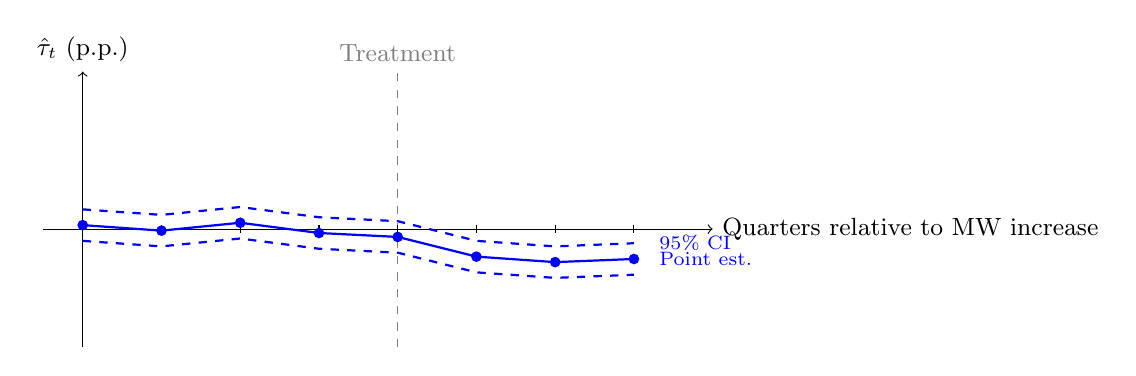
\begin{tikzpicture}[scale=1.0]
  \draw[->] (-0.5,0) -- (8,0) node[right] {\small Quarters relative to MW increase};
  \draw[->] (0,-1.5) -- (0,2) node[above] {\small $\hat{\tau}_t$ (p.p.)};
  \draw[dashed,gray] (4,-1.5) -- (4,2);
  \node[above,gray] at (4,2) {\small Treatment};
  \foreach \x in {0,1,...,7} \draw (\x,0.05) -- (\x,-0.05);
  \draw[thick,blue,mark=*,mark size=1.5pt] plot coordinates {(0,0.05) (1,-0.02) (2,0.08) (3,-0.05) (4,-0.1) (5,-0.35) (6,-0.42) (7,-0.38)};
  \draw[thick,blue,dashed] plot coordinates {(0,0.25) (1,0.18) (2,0.28) (3,0.15) (4,0.1) (5,-0.15) (6,-0.22) (7,-0.18)};
  \draw[thick,blue,dashed] plot coordinates {(0,-0.15) (1,-0.22) (2,-0.12) (3,-0.25) (4,-0.3) (5,-0.55) (6,-0.62) (7,-0.58)};
  \node[blue,right] at (7.2,-0.38) {\scriptsize Point est.};
  \node[blue,right] at (7.2,-0.18) {\scriptsize 95\% CI};
\end{tikzpicture}

\subsection{Robustness}

We conduct several robustness checks:

\begin{enumerate}
  \item Varying the pre-treatment window from 8 to 16 quarters.
  \item Excluding states with concurrent policy changes (e.g., earned income tax credit expansions).
  \item Using the ridge-augmented synthetic control of \citet{ben2021augmented}.
  \item Restricting the donor pool to states with no minimum wage changes during the sample period.
\end{enumerate}

All specifications yield qualitatively similar results. The youth unemployment effect remains significant across all robustness checks, while the aggregate effect remains insignificant.

\section{Conclusion}

This paper provides new evidence on the employment effects of minimum wage increases using the synthetic control method. Our findings are consistent with a monopsonistic labor market in which moderate minimum wage increases have limited aggregate disemployment effects but measurable impacts on youth employment. These results suggest that policymakers should consider age-specific labor market consequences when designing minimum wage legislation.

\bibliography{references}
\bibliographystyle{aer}

\end{document}
